
\chapter{Elettroni in un Potenziale Debole}

\section{Nearly-Free Electron Approximation}
In questa approssimazione il potenziale \( U(\mathbf{r}) \) tra gli elettroni e gli ioni è considerato debole. Le ragioni per poter adottare questo modello sono le seguenti:
\begin{itemize}
	\item L'interazione ione--elettrone è forte quando i due sono molto vicini, ma agli elettroni in conduzione non è permesso avvicinarsi troppo allo ione perché la regione attorno allo ione è già occupata dagli elettroni di core.
	\item Nella regione in cui sono permessi gli elettroni in conduzione la loro elevata mobilità permette uno screening efficace del campo generato dagli ioni, riducendo il potenziale netto che ciascun elettrone "sente".
\end{itemize}
Poiché il potenziale è debole, lo trattiamo come una perturbazione.
La funzione d'onda di Bloch si scrive come:
\[
\psi_{\mathbf{k}}(\mathbf{r}) = \sum_{K} c_{\mathbf{k}-\mathbf{K}}\, e^{i (\mathbf{k}-\mathbf{K})\cdot \mathbf{r}}\,,
\]
dove la somma viene effettuata su tutti i vettori del reticolo reciproco \(\mathbf{K}\).
I coefficienti \(c_{\mathbf{k}-\mathbf{K}}\) e l'energia \(\varepsilon\) sono determinati dall'hamiltoniana perturbata:
\begin{equation}
\left[ \frac{\hbar^2}{2m} (\mathbf{k} - \mathbf{K})^2 - \varepsilon \right] c_{\mathbf{k}-\mathbf{K}} + \sum_{K'} U_{\mathbf{K'}- \mathbf{K}} \, c_{\mathbf{k}-\mathbf{K'}} = 0\,.
\label{eqn:hampotdebole}
\end{equation}
La parte di perturbazione, dovuta al potenziale debole, è data dal termine:
\begin{equation}
\sum_{K'} U_{\mathbf{K'}- \mathbf{K}} \, c_{\mathbf{k}-\mathbf{K'}}\,.
\label{eqn:perturbazione}
\end{equation}
1) Per prima cosa risolviamo il \textbf{caso non perturbato, cioè per gli elettroni liberi}. \\
In assenza di \(U\) l'hamiltoniana si riduce a:
\[
\left[ \frac{\hbar^2}{2m}(\mathbf{k}-\mathbf{K})^2 - \varepsilon \right] c_{\mathbf{k}-\mathbf{K}} = 0\,.
\]
Definiamo l'energia degli elettroni liberi come:
\begin{equation}
\varepsilon^0_{\mathbf{q}} = \frac{\hbar^2 q^2}{2m}\,,
\label{eqn:enimpert}
\end{equation}
con \(\mathbf{q} = \mathbf{k} - \mathbf{K}\).
Pertanto, in assenza di perturbazione, l'equazione si scrive:
\[
(\varepsilon^0_{\mathbf{k}-\mathbf{K}} - \varepsilon)\, c_{\mathbf{k}-\mathbf{K}} = 0\,.
\]
Da questa equazione emergono due possibili soluzioni:
\begin{enumerate}
	\item \(c_{\mathbf{k}-\mathbf{K}} = 0\);
	\item Oppure \(\varepsilon = \varepsilon^0_{\mathbf{k}-\mathbf{K}}\).
\end{enumerate}
Nel caso \textbf{non degenere}, per un dato \(\mathbf{k}\) esiste un solo vettore \(\mathbf{K}_1\) per cui \(\varepsilon = \varepsilon^0_{\mathbf{k}-\mathbf{K}_1}\) e la funzione d'onda è proporzionale a \( e^{i(\mathbf{k}-\mathbf{K}_1)\cdot \mathbf{r}}\). \\\\

2) Nel caso \textbf{degenere} invece, si ha che per alcuni \(\mathbf{k}\) esistono più vettori del reticolo reciproco, \(\mathbf{K}_1, \ldots, \mathbf{K}_m\), tali che
\[
\varepsilon^0_{\mathbf{k}-\mathbf{K}_1} = \cdots = \varepsilon^0_{\mathbf{k}-\mathbf{K}_m}\,.
\]
In questo caso la soluzione è una combinazione lineare di onde piane:
\[
\psi_{\mathbf{k}}(\mathbf{r}) = \sum_{i=1}^{m} c_{\mathbf{k}-\mathbf{K}_i}\, e^{i(\mathbf{k}-\mathbf{K}_i)\cdot \mathbf{r}}\,.
\]
Poiché l'energia degli elettroni liberi è data dalla parabola \(\varepsilon^0_{\mathbf{q}} = \frac{\hbar^2 q^2}{2m}\), si ottengono delle parabole centrate in ciascun \(\mathbf{K}\) (vedi figura~\ref{fig:solpotdebole}).\\
L'unica soluzione indipendente si ottiene, per convenienza, nella prima zona di Brillouin, mentre i punti in cui due parabole si intersecano sono dei punti di degenerazione.

\begin{figure}[H]
	\centering
	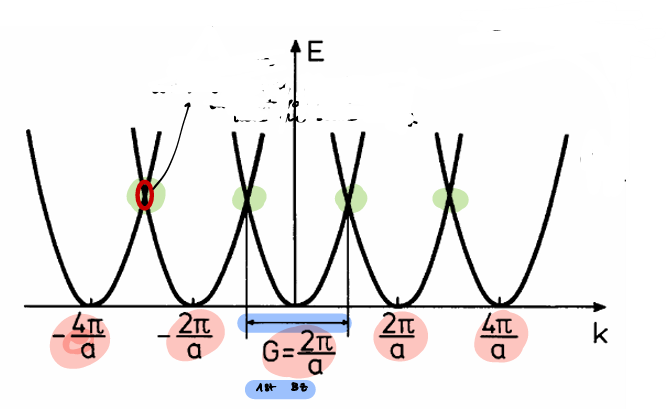
\includegraphics[width=\textwidth]{images/4-Elettroni-Potenziale-Debole/soluzpotdebole.png}
	\caption{Soluzioni imperturbate (onde piane) per il potenziale debole: parabole centrate in ciascun vettore \(\mathbf{K}\). I punti di intersezione rappresentano degenerazioni.}
	\label{fig:solpotdebole}
\end{figure}


\subsection{Effetti della Perturbazione Debole: Due Casi}
Quando il potenziale \(U\) non è più nullo occorrono correzioni all'energia e ai coefficienti \(c_{\mathbf{k}-\mathbf{K}}\).  
Esaminiamo due casi distinti:
\subsubsection{Caso A: Senza Degenerazione}

Fissato un certo \(\mathbf{k}\), supponiamo che esista un vettore \(\mathbf{K}_1\) tale che l'energia imperturbata \(\varepsilon^0_{\mathbf{k}-\mathbf{K}_1}\) sia ben separata (in termini dell'ordine di grandezza di \(U\)) da tutti gli altri livelli \(\varepsilon^0_{\mathbf{k}-\mathbf{K}}\) per ogni \(\mathbf{K} \neq \mathbf{K}_1\).  
Formalmente, si assume che
\begin{equation}
|\varepsilon^0_{\mathbf{k}-\mathbf{K}_1} - \varepsilon^0_{\mathbf{k}-\mathbf{K}}| \gg |U| \quad \text{per ogni } \mathbf{K} \neq \mathbf{K}_1\,.
\label{eqn:casoA}
\end{equation}
In questo caso la soluzione imperturbata è:
\[
\varepsilon = \varepsilon^0_{\mathbf{k}-\mathbf{K}_1}, \quad c_{\mathbf{k}-\mathbf{K}_1} \neq 0, \quad c_{\mathbf{k}-\mathbf{K}} = 0 \quad \text{per } \mathbf{K} \neq \mathbf{K}_1\,.
\]
Inserendo \( \mathbf{K} = \mathbf{K}_1 \) in \eqref{eqn:hampotdebole} si ottiene:
\begin{equation}
\bigl(\varepsilon - \varepsilon^0_{\mathbf{k}-\mathbf{K}_1}\bigr)c_{\mathbf{k}-\mathbf{K}_1} = \sum_{\mathbf{K}} U_{\mathbf{K} - \mathbf{K}_1} \, c_{\mathbf{k}-\mathbf{K}}\,.
\label{eqn:eq1}
\end{equation}
Si ricorda che la costante additiva del potenziale è scelta in modo tale che \(U_{\mathbf{0}} = 0\); pertanto, nel lato destro appariranno solo termini con \(\mathbf{K} \neq \mathbf{K}_1\).

Per \(\mathbf{K} \neq \mathbf{K}_1\), si può risolvere l'equazione \eqref{eqn:hampotdebole} per \(c_{\mathbf{k}-\mathbf{K}}\):
\[ c_{k - K} = \frac{U_{\mathbf{K}_1 - \mathbf{K}}\,c_{\mathbf{k}-\mathbf{K}_1}}{\varepsilon - \varepsilon^0_{\mathbf{k}-\mathbf{K}}}  + \sum_{K' \neq K_1}\frac{U_{K'-K}c_{k - K'}}{\varepsilon - \varepsilon^0_{k - K}}c_{\mathbf{k}-\mathbf{K}} = \frac{U_{\mathbf{K}_1 - \mathbf{K}}\,c_{\mathbf{k}-\mathbf{K}_1}}{\varepsilon - \varepsilon^0_{\mathbf{k}-\mathbf{K}}} + O(U^2)\]
Poiché per il caso non degenere (secondo l'ipotesi in \eqref{eqn:casoA}) \(\varepsilon^0_{\mathbf{k}-\mathbf{K}}\) è ben distante da \(\varepsilon^0_{\mathbf{k}-\mathbf{K}_1}\), i termini \(c_{\mathbf{k}-\mathbf{K}}\) risultano di ordine \(U\).  \\\\
Sostituendo nell'equazione per \(\mathbf{K} = \mathbf{K}_1\) in \eqref{eqn:eq1} si ottiene:
\[
\bigl(\varepsilon - \varepsilon^0_{\mathbf{k}-\mathbf{K}_1}\bigr)c_{\mathbf{k}-\mathbf{K}_1} = \sum_{\mathbf{K}\neq \mathbf{K}_1} U_{\mathbf{K} - \mathbf{K}_1}\, \frac{U_{\mathbf{K}_1-\mathbf{K}}\,c_{\mathbf{k}-\mathbf{K}_1}}{\varepsilon - \varepsilon^0_{\mathbf{k}-\mathbf{K}}} + O(U^3)\,.
\]
Dividendo per \(c_{\mathbf{k}-\mathbf{K}_1}\) (non nullo) e risolvendo per \(\varepsilon\) con le opportune simmetrie $U_k = U_{-k}= U^*_k$, si ottiene la correzione al secondo ordine:
\[
\varepsilon = \varepsilon^0_{\mathbf{k}-\mathbf{K}_1} + \sum_{\mathbf{K}\neq \mathbf{K}_1} \frac{|U_{\mathbf{K}_1-\mathbf{K}}|^2}{\varepsilon^0_{\mathbf{k}-\mathbf{K}_1} - \varepsilon^0_{\mathbf{k}-\mathbf{K}}} + O(U^3)\,.
\]
Questa espressione mostra che le bande non degenere subiscono uno spostamento (o "repulsione") perturbativo:  
i livelli imperturbati inferiori (con denominatore positivo) contribuiscono ad aumentare \(\varepsilon\) mentre quelli superiori (con denominatore negativo) tendono a diminuirla.
\begin{figure}[H]
	\centering
	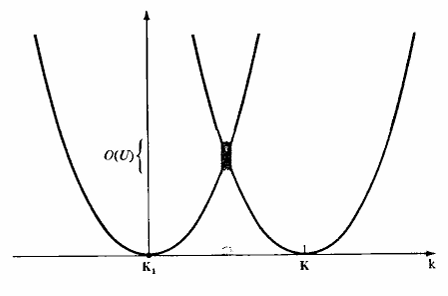
\includegraphics[width=0.5\textwidth]{images/4-Elettroni-Potenziale-Debole/seplivU.png}
	\caption{Intervallo di \(k\) in cui i livelli di energia imperturbati \(\varepsilon^0_{\mathbf{k}-\mathbf{K}_1}\) e \(\varepsilon^0_{\mathbf{k}-\mathbf{K}}\) differiscono di un termine dell'ordine \(O(U)\).}
	\label{fig:seplivU}
\end{figure}


\subsubsection{Caso B: Caso Degenere}
Supponiamo ora che, per un certo \(\mathbf{k}\), esistano \(m\) vettori del reticolo reciproco \(\mathbf{K}_1, \ldots, \mathbf{K}_m\) tali che:
\[
\varepsilon^0_{\mathbf{k}-\mathbf{K}_1} = \varepsilon^0_{\mathbf{k}-\mathbf{K}_2} = \cdots = \varepsilon^0_{\mathbf{k}-\mathbf{K}_m}\,,
\]
e che per ogni \(\mathbf{K} \not\in \{\mathbf{K}_1, \ldots, \mathbf{K}_m\}\) si abbia
\[
|\varepsilon^0_{\mathbf{k}-\mathbf{K}} - \varepsilon^0_{\mathbf{k}-\mathbf{K}_i}| \gg |U| \quad \text{per } i=1,\ldots,m\,.
\]
In questo caso le equazioni \eqref{eqn:hampotdebole} per \( \mathbf{K} = \mathbf{K}_i\) (con \(i=1,\ldots,m\)) devono essere trattate insieme.  
Per \(i=1,\ldots,m\) scriviamo:
\begin{equation}
\bigl(\varepsilon - \varepsilon^0_{\mathbf{k}-\mathbf{K}_i}\bigr)c_{\mathbf{k}-\mathbf{K}_i} = \sum_{j=1}^{m} U_{\mathbf{K}_j-\mathbf{K}_i}\, c_{\mathbf{k}-\mathbf{K}_j} + \sum_{\mathbf{K} \notin \{\mathbf{K}_1,\ldots,\mathbf{K}_m\}} U_{\mathbf{K}-\mathbf{K}_i}\, c_{\mathbf{k}-\mathbf{K}}\,,
\label{eqn:eq4}
\end{equation}
mentre per \(\mathbf{K}\) al di fuori dell'insieme degenere abbiamo (come nel caso A):
\begin{equation}
c_{\mathbf{k}-\mathbf{K}} = \frac{1}{\varepsilon - \varepsilon^0_{\mathbf{k}-\mathbf{K}}} \sum_{j=1}^{m} U_{\mathbf{K}_j-\mathbf{K}}\, c_{\mathbf{k}-\mathbf{K}_j} + O(U^2)\,,
\label{eqn:eq3}
\end{equation}
il cui contributo è di ordine \(U\).  
Inserendo \eqref{eqn:eq3} nell'equazione (\ref{eqn:eq4}) per \(i=1,\ldots,m\), il termine perturbativo esterno fornisce contributi di ordine \(U^2\).  
Dal momento che stiamo ricercando gli effetti principali, e considerando che nel limite \(U\to 0\) tale termine diventa trascurabile, trunchiamo al primo ordine ottenendo il sistema lineare:
\begin{equation}
\bigl(\varepsilon - \varepsilon^0_{\mathbf{k}-\mathbf{K}_i}\bigr) c_{\mathbf{k}-\mathbf{K}_i} = \sum_{j=1}^{m} U_{\mathbf{K}_j-\mathbf{K}_i}\, c_{\mathbf{k}-\mathbf{K}_j}, \quad i=1,\ldots,m\,.
\label{eqn:eq6}
\end{equation}
Questo sistema di \(m\) equazioni lineari determina i coefficienti \(c_{\mathbf{k}-\mathbf{K}_i}\) e le energie perturbate \(\varepsilon\) entro il sottospazio di degenerazione.  
L'energia risultante subirà uno spostamento del secondo ordine in \(U\); tuttavia, in questo trattamento di base, il problema si riduce alla diagonalizzazione della matrice perturbativa \(U_{\mathbf{K}_j-\mathbf{K}_i}\) al fine di determinare le correzioni energetiche.

Riassumendo:
\begin{itemize}
	\item Nel \textbf{caso non degenere} (condizione \eqref{eqn:casoA}), l'energia perturbata è data da:
	\[
	\varepsilon = \varepsilon^0_{\mathbf{k}-\mathbf{K}_1} + \sum_{\mathbf{K} \neq \mathbf{K}_1} \frac{|U_{\mathbf{K}_1-\mathbf{K}}|^2}{\varepsilon^0_{\mathbf{k}-\mathbf{K}_1} - \varepsilon^0_{\mathbf{k}-\mathbf{K}}} + O(U^3)\,.
	\]
	\item Nel \textbf{caso degenere}, il problema si riduce a diagonalizzare la matrice perturbativa \(U_{\mathbf{K}_j-\mathbf{K}_i}\) all'interno del sottospazio degenerato, determinando così le energie perturbate e la combinazione lineare degli stati che, in assenza di \(U\), risultavano degenere.
\end{itemize}

Questo trattamento permette di comprendere come il potenziale debole, trattato come perturbazione, modifichi i livelli energetici degli elettroni. Nei casi non degeneri l'effetto della perturbazione compare al secondo ordine, mentre nei casi degenere la struttura degli autostati viene "mista" e si ottengono soluzioni linearmente combinate che eliminano la degenerazione.

\bigskip






\section{Livelli Energetici Vicino ai Piani di Bragg}
In questa sezione si analizzano le soluzioni dell'equazione agli autovalori per elettroni in un potenziale periodico debole, concentrandosi sui casi in cui due livelli dell'elettrone libero sono quasi degeneri, ovvero quando la loro energia imperturbata differisce di un termine dell'ordine di \(U\) (l'ampiezza del potenziale perturbativo), mentre la differenza con gli altri livelli è molto maggiore di \(U\).  
Formalmente, supponiamo che per una certa quantità \(\mathbf{q}\) (dove \(\mathbf{q} = \mathbf{k} - \mathbf{K}_1\)) si abbia
\[
\varepsilon^0_{q} \sim \varepsilon^0_{q-K}\,,
\]
con la condizione che per ogni altro vettore di reticolo \(\mathbf{K'} \neq 0,\) si verifichi:
\[
|\varepsilon^0_{q} - \varepsilon^0_{q-K'}| \gg |U|\,.
\]
Questa condizione si verifica quando
\[
|q| = |q-K|\,,
\]
che è la definizione geometrica di un piano di Bragg.\\
Da ciò possiamo dedurre due affermazioni fondamentali:
\begin{itemize}
	\item Se \(|q| = |q-K|\), allora il punto \(\mathbf{q}\) giace sul piano di Bragg determinato dal vettore di reticolo \(K\).
	\item Se il punto \(\mathbf{q}\) giace sul piano di Bragg, allora il vettore \(\mathbf{q} - \frac{1}{2}\mathbf{K}\) è parallelo al piano.
\end{itemize}
(Per ulteriori dettagli, si veda la sezione denominata “Formulazione di Von Laue”.)\\\\
Le figure in basso mostrano due rappresentazioni grafiche degli stati energetici vicino al piano di Bragg:
\begin{figure}[H]
	\centering
	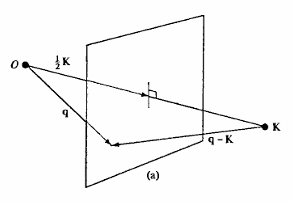
\includegraphics[width=0.4\textwidth]{images/4-Elettroni-Potenziale-Debole/elevelBraggP1.png}
	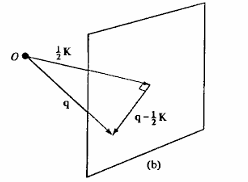
\includegraphics[width=0.4\textwidth]{images/4-Elettroni-Potenziale-Debole/elevelBraggP2.png}
	\caption{Diagrammi schematici dei livelli energetici vicino al piano di Bragg.}
	\label{fig:elevelBraggP}
\end{figure}

\bigskip
\noindent
\textbf{ Ci si aspetta degenerazione al bordo della zona di Brillouin, in quanto i vettori d'onda di elettroni vicini ai piani di Bragg, dove si possono verificare riflessioni di Bragg, sono quelli maggiormente influenzati dal potenziale periodico debole.}\\
\bigskip
\subsection{Struttura dei Livelli quando un Solo Piano di Bragg è Vicino}
Consideriamo il caso in cui un solo piano di Bragg interferisca con i livelli imperturbati. Supponiamo di avere due componenti significative per la funzione d'onda, associate a due vettori del reticolo reciproco \(K_1\) e \(K_2\). In assenza di perturbazione le energie imperturbate sono:
\[
\varepsilon^0_{k-K_1} \quad \text{e} \quad \varepsilon^0_{k-K_2}\,,
\]
ed ipotizziamo che siano quasi degeneri. L'equazione perturbata (vedi equazione \eqref{eqn:hampotdebole} della sezione precedente) assume, per i due termini significativi, la forma:
\[
(\varepsilon - \varepsilon^0_{k-K_1})\,c_{k-K_1} = U_{K_2 - K_1}\,c_{k-K_2}\,,
\]
\[
(\varepsilon - \varepsilon^0_{k-K_2})\,c_{k-K_2} = U_{K_1 - K_2}\,c_{k-K_1}\,.
\]
Per semplificare l'analisi, introduciamo le nuove variabili:
\[
q = k-K_1,\quad \text{e} \quad K = K_2 - K_1\,.
\]
Con queste definizioni, le due equazioni diventano:
\begin{equation}
(\varepsilon - \varepsilon^0_{q})\, c_{q} = U_{K}\, c_{q-K}\,,
\label{eqn:eqBragg}
\end{equation}
\begin{equation}
(\varepsilon - \varepsilon^0_{q-K})\, c_{q-K} = U_{-K}\, c_{q}\,.
\label{eqn:eqBragg2}
\end{equation}
Per trovare le energie permettendo la presenza di due componenti, cerchiamo soluzioni non banali imponendo che il sistema omogeneo di equazioni abbia determinante nullo:
\[
\det \begin{pmatrix}
\varepsilon - \varepsilon^0_{q} & -U_{K} \\
-U_{K}^* & \varepsilon - \varepsilon^0_{q-K}
\end{pmatrix} = 0\,.
\]
Questo determinante fornisce:
\[
(\varepsilon - \varepsilon^0_{q})(\varepsilon - \varepsilon^0_{q-K}) - |U_K|^2 = 0\,.
\]
Risolvendo per \(\varepsilon\) si ottiene:
\begin{equation}
\varepsilon = \frac{1}{2}\left(\varepsilon^0_{q} + \varepsilon^0_{q-K}\right) \pm \sqrt{\left(\frac{\varepsilon^0_{q} - \varepsilon^0_{q-K}}{2}\right)^2 + |U_K|^2}\,.
\label{eqn:soluzioneeps}
\end{equation}
Nel caso particolare in cui il punto \(q\) giaccia sul piano di Bragg, abbiamo
\[
|q| = |q-K| \quad \Rightarrow \quad \varepsilon^0_{q} = \varepsilon^0_{q-K}\,.
\]
Quindi l'equazione \eqref{eqn:soluzioneeps} si semplifica a:
\[
\varepsilon = \varepsilon^0_{q} \pm |U_K|\,.
\]
Questo risultato mostra che, in corrispondenza del piano di Bragg, l'energia si splitta in due valori differenti separati da un gap di ampiezza \(2|U_K|\).\\
Inoltre, ricordando che per un elettrone libero
\[
\varepsilon^0_q = \frac{\hbar^2 q^2}{2m}\,,
\]
si calcola il gradiente dell'energia:
\[
\frac{\partial \varepsilon}{\partial q} = \frac{\hbar^2}{m}\left(q - \frac{1}{2}K\right)\,.
\]
Si osserva che il gradiente risulta parallelo al piano di Bragg (poiché \(K\) è fisso per quel piano).\\\\
\textbf{Determinazione delle Funzioni d'Onda:}
Per il sistema di equazioni \eqref{eqn:eqBragg} e \eqref{eqn:eqBragg2} risulta utile analizzare il rapporto tra i coefficienti \(c_q\) e \(c_{q-K}\).  
Se poniamo:
\[
\varepsilon = \varepsilon^0_q \pm |U_K|\,,
\]
l'equazione \eqref{eqn:eqBragg} diventa (notando che \(\varepsilon - \varepsilon^0_q = \pm |U_K|\)):
\[
\pm |U_K|\, c_{q} = U_K\, c_{q-K}\,,
\]
da cui si ricava:
\[
c_{q} = \pm \frac{U_K}{|U_K|}\, c_{q-K} = \pm \operatorname{sgn}(U_K)\, c_{q-K}\,.
\]
Pertanto, a seconda del segno di \(U_K\), le due soluzioni avranno coefficienti in rapporto:
\begin{itemize}
	\item Per \(U_K>0\):
		\[
		|\psi(r)|^2 \propto \left(\cos\frac{1}{2}K\cdot r\right)^2 \quad \text{per } \varepsilon = \varepsilon^0_q + |U_K|,
		\]
		\[
		|\psi(r)|^2 \propto \left(\sin\frac{1}{2}K\cdot r\right)^2 \quad \text{per } \varepsilon = \varepsilon^0_q - |U_K|.
		\]
	\item Per \(U_K<0\):
		\[
		|\psi(+)|^2 \propto \left(\sin\frac{1}{2}K\cdot r\right)^2 \quad \text{per } \varepsilon = \varepsilon^0_q + |U_K|,
		\]
		\[
		|\psi(-)|^2 \propto \left(\cos\frac{1}{2}K\cdot r\right)^2 \quad \text{per } \varepsilon = \varepsilon^0_q - |U_K|.
		\]
\end{itemize}
La figura~\ref{fig:andamentiUpsi} mostra schematicamente l'andamento delle funzioni d'onda corrispondenti ai due livelli (le soluzioni sono "piccate" rispettivamente sull'atomo e nello spazio tra gli atomi).
\begin{figure}[H]
	\centering
	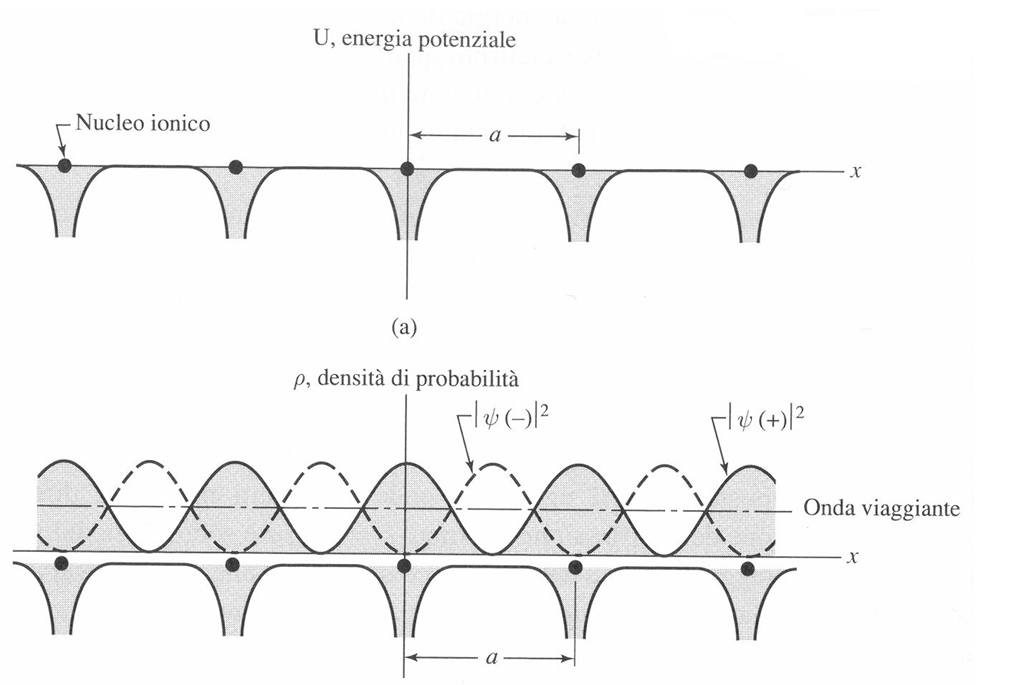
\includegraphics[width=0.8\textwidth]{images/4-Elettroni-Potenziale-Debole/andamentiUpsi.png}
	\caption{Le funzioni d'onda \(|\psi(+)|^2\) e \(|\psi(-)|^2\) per i due livelli splitati. La soluzione \(|\psi(+)|^2\) presenta massimo di densità sull'atomo, mentre \(|\psi(-)|^2\) è massima negli spazi interatomo.}
	\label{fig:andamentiUpsi}
\end{figure}

\bigskip
\subsection{Bande Energetiche in una Dimensione}
È utile illustrare come si presentano i livelli energetici nel caso monodimensionale, in modo da evidenziare il ruolo dei piani di Bragg nella separazione (splitting) dei livelli.\\\\
\textbf{(i) Caso Elettrone Libero:}  
In assenza di interazioni il grafico dell'energia in funzione di \(k\) è una parabola:
\begin{figure}[H]
	\centering
	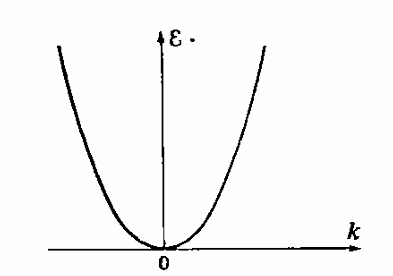
\includegraphics[width=0.4\textwidth]{images/4-Elettroni-Potenziale-Debole/livellien1Da.png}
	\caption{Livelli energetici di un elettrone libero (parabola).}
	\label{fig:livellien1Da}
\end{figure}

\textbf{(ii) Con Potenziale Periodico Debole:}  
La parabola dell'elettrone libero resta valida eccetto nelle vicinanze dei piani di Bragg.  
Quando \(q\) è vicino al piano di Bragg corrispondente a un vettore di reticolo \(K\), l'energia corretta si ottiene disegnando parabole centrate in \(K\).  
Questa rappresentazione è mostrata nella figura:
\begin{figure}[H]
	\centering
	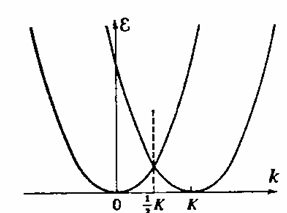
\includegraphics[width=0.4\textwidth]{images/4-Elettroni-Potenziale-Debole/livellien1Db.png}
	\caption{Livelli energetici in presenza di un potenziale periodico debole: parabole traslate.}
	\label{fig:livellien1Db}
\end{figure}

Al punto di intersezione delle parabole (piano di Bragg) la degenerazione viene risolta (split) di un ammontare pari a \(2|U_K|\) in modo che la derivata dell'energia sia nulla in quel punto. La figura successiva mostra la riproiezione con il gap:
\begin{figure}[H]
	\centering
	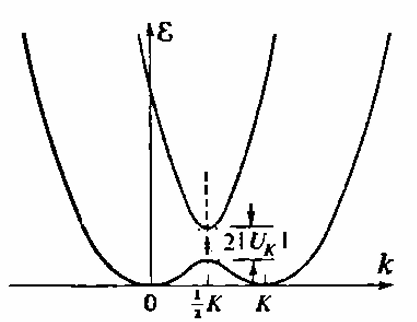
\includegraphics[width=0.4\textwidth]{images/4-Elettroni-Potenziale-Debole/livellien1Dc.png}
	\caption{Splitting delle parabole nelle vicinanze di un piano di Bragg.}
	\label{fig:livellien1Dc}
\end{figure}

La curva originale del caso libero (Figura~\ref{fig:livellien1Da}) si trasforma nella rappresentazione che si ottiene includendo l'effetto del potenziale (Figura~\ref{fig:livellien1Db}).  
Per visualizzare l'intera struttura a bande, si procede poi ad un'estensione nel cosiddetto \textbf{extended-zone scheme}, in cui ogni banda viene rappresentata nella propria zona di Brillouin:
\begin{figure}[H]
	\centering
	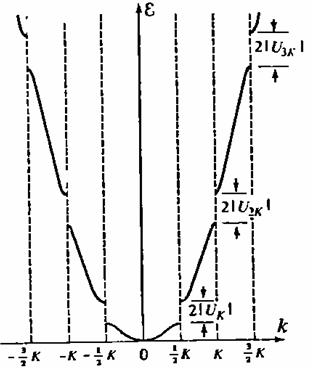
\includegraphics[width=0.4\textwidth]{images/4-Elettroni-Potenziale-Debole/livellien1De.png}
	\caption{Extended-zone scheme: ogni banda viene rappresentata nella corrispettiva zona di Brillouin.}
	\label{fig:livellien1De}
\end{figure}

Esistono schemi alternativi, come il \textbf{reduced zone scheme} (in cui tutte le bande vengono "riportate" nella prima zona di Brillouin) e il \textbf{repeated zone scheme}. Ad esempio, la figura seguente confronta i due schemi:
\begin{figure}[H]
	\centering
	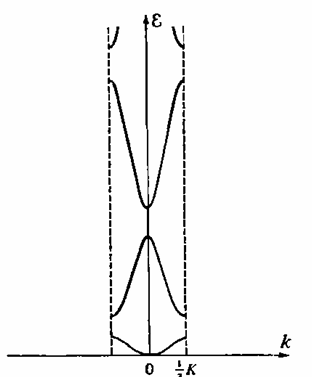
\includegraphics[width=0.4\textwidth]{images/4-Elettroni-Potenziale-Debole/reduced.png}
	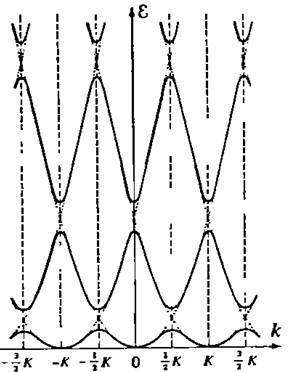
\includegraphics[width=0.4\textwidth]{images/4-Elettroni-Potenziale-Debole/repeated.png}
	\caption{A sinistra il reduced zone scheme, a destra il repeated zone scheme.}
	\label{fig:redrep}
\end{figure}

Infine, se il vettore di Fermi \(k_F\) si trova, ad esempio, tra \(-K\) e \(-\frac{1}{2}K\), dalla conoscenza di \(k_F\) è possibile dedurre immediatamente quante bande siano riempite.

\bigskip
\subsection{Bande Energetiche in Tre Dimensioni}
In tre dimensioni le bande energetiche, ottenute dalla soluzione dell'equazione agli autovalori per elettroni in un potenziale periodico, assumono forme complesse.  \\
Ad esempio, in un reticolo fcc privo di interazioni il grafico delle bande mostra punti di degenerazione in corrispondenza di punti specifici (ad es. il punto X) e il punto \(\Gamma\) rappresenta il centro della prima zona di Brillouin:
\begin{figure}[H]
	\centering
	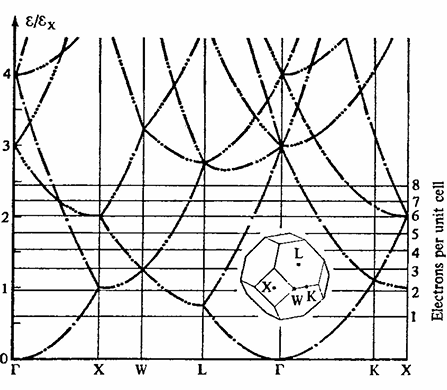
\includegraphics[width=0.6\textwidth]{images/4-Elettroni-Potenziale-Debole/bande3d1.png}
	\caption{Bande energetiche in 3D per un reticolo fcc senza interazioni.}
	\label{fig:bande3d1}
\end{figure}

Nel caso di materiali con interazioni (ad es. il silicio) la struttura a bande risulta modificata: in alcuni punti del reticolo reciproco (come X) possono rimanere degenerazioni mentre in altri (ad es. \(L\)) si apre un gap:
\begin{figure}[H]
	\centering
	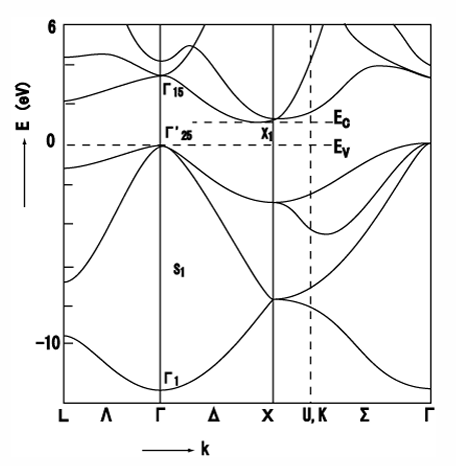
\includegraphics[width=0.6\textwidth]{images/4-Elettroni-Potenziale-Debole/bande3d2.png}
	\caption{Bande energetiche del silicio: si evidenziano gap e degenerazioni in diversi punti del reticolo reciproco.}
	\label{fig:bande3d2}
\end{figure}

\bigskip
\section{Zone di Brillouin}
Utilizzando la teoria degli elettroni in un potenziale, risulta possibile determinare l'intera struttura a bande tridimensionale di un cristallo.  
Si osserva che la posizione del vettore d'onda di Fermi fornisce informazioni sulle bande occupate:  
\begin{itemize}
	\item Se la superficie di Fermi imperturbata è completamente contenuta all'interno di una zona di Brillouin, allora la banda corrispondente è piena o parzialmente piena.
	\item Se invece la superficie di Fermi "spunta" da una zona di Brillouin (ovvero si trova tra due bande), la banda superiore risulterà vuota mentre quella inferiore sarà piena.
\end{itemize}
La figura seguente mostra le diverse zone di Brillouin per vari tipi di cristalli:
\begin{figure}[H]
	\centering
	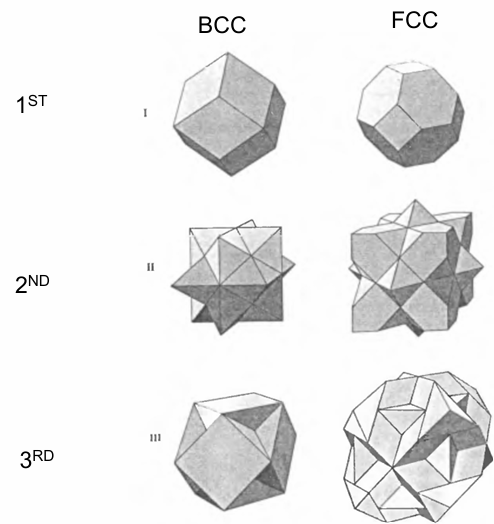
\includegraphics[width=0.6\textwidth]{images/4-Elettroni-Potenziale-Debole/zonediBr.png}
	\caption{Zone di Brillouin per diversi tipi di cristalli.}
	\label{fig:zonedibr}
\end{figure}


\bigskip
\section{Il Fattore di Struttura Geometrica in Reticoli con Base}
Quando il cristallo presenta più di un atomo per cella unitaria, il potenziale periodico derivante dagli ioni assume la forma
\[
U(\mathbf{r}) = \sum_{\mathbf{R}} \sum_j \phi\Bigl(\mathbf{r} - \mathbf{R} - \mathbf{d}_j\Bigr)\,,
\]
dove:
\begin{itemize}
	\item \(\mathbf{R}\) rappresenta il vettore di traslazione della cella unitaria,
	\item \(j\) scorre sugli atomi contenuti nella cella, che si trovano nelle posizioni \(\mathbf{d}_j\).
\end{itemize}
La componente Fourier del potenziale (cioè, la sua rappresentazione in \(\mathbf{K}\)-space) è definita da:
\[
U_{\mathbf{K}} = \frac{1}{v} \int_{\text{cella}} \d\mathbf{r}\, e^{-i\mathbf{K}\cdot\mathbf{r}}\, U(\mathbf{r})\,,
\]
dove \(v\) è il volume della cella unitaria.  
Inserendo l'espressione per \(U(\mathbf{r})\), si ha:
\[
U_{\mathbf{K}} = \frac{1}{v} \int_{\text{cella}} \d\mathbf{r}\, e^{-i\mathbf{K}\cdot\mathbf{r}} \sum_{\mathbf{R}} \sum_j \phi\Bigl(\mathbf{r} - \mathbf{R} - \mathbf{d}_j\Bigr)\,.
\]
Osserviamo che, poiché \(\phi(\mathbf{r})\) è un potenziale locale (importante solo in prossimità di ogni ione), la sommatoria sull'insieme delle traslazioni \(\mathbf{R}\) permette di estendere l'integrazione dalla cella unitaria a tutto lo spazio:
\[
U_{\mathbf{K}} = \frac{1}{v} \int_{\mathbb{R}^3} \d\mathbf{r}\, e^{-i\mathbf{K}\cdot\mathbf{r}} \sum_j \phi\Bigl(\mathbf{r} - \mathbf{d}_j\Bigr)\,.
\]
Definiamo quindi la trasformata di Fourier del potenziale locale:
\[
\phi(\mathbf{K}) = \int_{\mathbb{R}^3} \d\mathbf{r}\, e^{-i\mathbf{K}\cdot\mathbf{r}}\, \phi(\mathbf{r})\,,
\]
e il \emph{fattore di struttura}:
\[
S_{\mathbf{K}} = \sum_j e^{i\mathbf{K}\cdot\mathbf{d}_j}\,.
\]
Con queste definizioni la componente Fourier del potenziale risulta:
\[
U_{\mathbf{K}} = \frac{1}{v}\, \phi(\mathbf{K})\, S_{\mathbf{K}}^*\,.
\]
Riassumendo, il potenziale periodico in un reticolo con base si scrive come:
\[
\boxed{ U_{\mathbf{K}} = \frac{1}{v}\, \phi(\mathbf{K})\, S_{\mathbf{K}}^* \quad \text{con} \quad \phi(\mathbf{K}) = \int_{\mathbb{R}^3} \d\mathbf{r}\, e^{-i\mathbf{K}\cdot\mathbf{r}}\, \phi(\mathbf{r}), \quad S_{\mathbf{K}} = \sum_j e^{i\mathbf{K}\cdot\mathbf{d}_j}\,. }
\]
Questo risultato evidenzia che il potenziale Fourier \(U_{\mathbf{K}}\) è dato dal prodotto della forma del potenziale locale (tramite \(\phi(\mathbf{K})\)) e del fattore di struttura, che riflette la disposizione geometrica degli atomi nella cella unitaria.
